\section{Generators}

By sequentially or horizontally composing the \textit{Z Spider} (green) and \textit{X Spider} (red) generators, we can construct undirected multigraphs known as ZX diagrams \cite{Wetering2020}. That is, graphs that allow multiple edges between vertices. Since \textit{only connectivity matters} in the ZX calculus, a valid ZX diagram can be arbitrarily deformed (\textit{d}), provided that the order of inputs and outputs is preserved.

\begin{figure}[H]
\centering
    \centering
    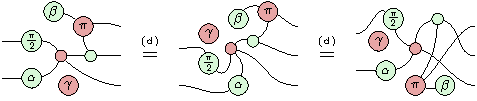
\includegraphics[width=0.8\textwidth]{chapter-2/connectivity}
    \caption{Three equivalent ZX diagrams (\textit{only connectivity matters}).}
    \label{only-connectivity-matters}
\end{figure}

\notation{We interpret the flow of time left to right. Hence, the wires on the left refer to inputs and the wires on the right refer to outputs.}

Z Spiders (green) are defined with respect to the $Z$ eigenbasis ($\ket 0$ and $\ket 1$) such that a Z Spider with $n$ inputs and $m$ outputs represents the following linear map.

\begin{figure}[H]
\centering
\includezxdiagramtext{figures/chapter-2/z_spider}{0.21}{\,
    \ket{0}^{\otimes m} \bra{0}^{\otimes n} + e^{i\alpha}
    \ket{1}^{\otimes m} \bra{1}^{\otimes n}}
\caption{Interpretation of a Z Spider as a linear map.}
\end{figure}

$X$ Spiders (red), are defined with respect to the $X$ eigenbasis ($\ket +$ and $\ket -$).

\begin{figure}[H]
\centering
\includezxdiagramtext{figures/chapter-2/x_spider}{0.21}{\,
    \ket{+}^{\otimes m} \bra{+}^{\otimes n} + e^{i\alpha}
    \ket{-}^{\otimes m} \bra{-}^{\otimes n}}
\caption{Interpretation of an X Spider as a linear map.}
\end{figure}

We can represent the $Z$ eigenstates, $\ket 0$ and $\ket 1$, using an $X$ spider with a phase of either $0$ or $\pi$.

\begin{figure}[H]
\centering
\begin{minipage}{.4\textwidth}
    \centering
    \includezxdiagramtext{figures/chapter-2/zero_state}{0.15}{\,
        \ket + + \ket - = \sqrt{2} \ket 0}
    \caption{$\ket 0$ eigenstate}
\end{minipage}%
\begin{minipage}{.4\textwidth}
    \centering
    \includezxdiagramtext{figures/chapter-2/one_state}{0.16}{\,
    \ket + - \ket - = \sqrt{2} \ket 1}
    \caption{$\ket 1$ eigenstate}
\end{minipage}
\end{figure}

Similarly, we can represent the $X$ eigenstates, $\ket +$ and $\ket -$, using the corresponding $Z$ spiders.

\begin{figure}[H]
\centering
\begin{minipage}{.4\textwidth}
    \centering
    \includezxdiagramtext{figures/chapter-2/plus_state}{0.15}{\,
        \ket 0 + \ket 1 = \sqrt{2} \ket +}
    \caption{$\ket +$ eigenstate}
\end{minipage}%
\begin{minipage}{.4\textwidth}
    \centering
    \includezxdiagramtext{figures/chapter-2/minus_state}{0.16}{\,
    \ket 0 - \ket 1 = \sqrt{2} \ket -}
    \caption{$\ket -$ eigenstate}
\end{minipage}
\end{figure}

Single qubit rotations in the $Z$ basis are represented by a Z Spider with a single input and a single output. Arbitrary rotations in the $X$ basis are represented by the corresponding $X$ spider. We can view these as rotations of the Bloch sphere.

\includezxdiagramtextplus{figures/chapter-2/z_rotation}{0.11}{
    \ket{0} \bra{0} + e^{i\alpha}
    \ket{1} \bra{1} = 
    \begin{pmatrix} 1 & 0 \\ 0 & e^{i\alpha} \end{pmatrix}
    \rightarrow
}
{chapter-1/z_rotation}{0.18}
\vspace*{-15pt}
\includezxdiagramtextplus{figures/chapter-2/x_rotation}{0.11}{
    \ket{+} \bra{+} +
    e^{i\alpha} \ket{-} \bra{-} = 
    \frac{1}{2} \begin{pmatrix}
    1 + e^{i\alpha} & 1 - e^{i\alpha} \\
    1 - e^{i\alpha} & 1 + e^{i\alpha}
    \end{pmatrix}
    \rightarrow
}
{chapter-1/x_rotation}{0.17}

We can recover the Pauli $Z$ and Pauli $X$ matrices by setting the angle $\alpha = \pi$.

\begin{figure}[H]
\centering
\includezxdiagramtext{figures/chapter-2/pauli_z}{0.11}{
    \ket{0} \bra{0} + e^{i\pi} \ket{1} \bra{1} = 
    \begin{pmatrix} 1 & \,\,0 \\ 0 & -1 \end{pmatrix}
}
\includezxdiagramtext{figures/chapter-2/pauli_x}{0.11}{
    \ket{+} \bra{+} + e^{i\pi} \ket{-} \bra{-} = 
    \begin{pmatrix} 0 & 1 \\ 1 & 0 \end{pmatrix}
}
\caption{Pauli $Z$ and $X$ gates in the ZX calculus.}
\end{figure}

%%%

\subsection{Composition}%
\label{composition}

To calculate the matrix of a ZX diagram consisting of sequentially composed spiders, we take the matrix product. Note that the order of operation of matrix multiplication is the reverse as in the ZX diagram as we have defined it.

\includezxdiagramtext{chapter-2/sequential}{0.27}{
\begin{pmatrix} 1 & 0 \\ 0 & e^{i\gamma} \end{pmatrix}
\begin{pmatrix}
    1 + e^{i\beta} & 1 - e^{i\beta} \\
    1 - e^{i\beta} & 1 + e^{i\beta}
\end{pmatrix}
\begin{pmatrix} 1 & 0 \\ 0 & e^{i\alpha} \end{pmatrix}}

Alternatively, we could have chosen to compose the spiders in parallel, resulting in the tensor product.

\includezxdiagramtext{chapter-2/parallel}{0.105}{
\begin{pmatrix} 1 & 0 \\ 0 & e^{i\alpha} \end{pmatrix} \otimes
\begin{pmatrix}
    1 + e^{i\beta} & 1 - e^{i\beta} \\
    1 - e^{i\beta} & 1 + e^{i\beta}
\end{pmatrix}}

The CNOT gate in the ZX calculus is represented by a Z spider (control qubit) and an X spider (target qubit). We can arbitrarily deform the diagram and decompose it into matrix and tensor products as follows.

\includezxdiagram{chapter-2/cnot_def}{0.65}

We can calculate matrix $A$, consisting of a single-input and two-output Z Spider ($4 \times 2$ matrix) and an empty wire (identity matrix), by taking the tensor product.

\includezxdiagramtext{chapter-2/A_def}{0.33}{
\begin{pmatrix}
    1 & 0 \\
    0 & 0 \\
    0 & 0 \\
    0 & 1
\end{pmatrix} \otimes
\begin{pmatrix} 1 & 0 \\ 0 & 1 \end{pmatrix}}

Similarly, to calculate the matrix $B$, we take the following tensor product.

\includezxdiagramtext{chapter-2/B_def}{0.33}{
\begin{pmatrix} 1 & 0 \\ 0 & 1 \end{pmatrix} \otimes \frac{1}{\sqrt 2}
\begin{pmatrix} 1 & 0 & 0 & 1 \\ 0 & 1 & 1 & 0 \end{pmatrix}}

We can then calculate the CNOT matrix by taking the matrix product of matrix $A$ and matrix $B$ as follows.

\includezxdiagramtext{chapter-2/cnot}{0.10}{
    \Bigg[
    \begin{pmatrix} 1 & 0 \\ 0 & 1 \end{pmatrix} \otimes \frac{1}{\sqrt 2}
    \begin{pmatrix} 1 & 0 & 0 & 1 \\ 0 & 1 & 1 & 0 \end{pmatrix} \Bigg]
    %
    \left[ \begin{pmatrix}
        1 & 0 \\
        0 & 0 \\
        0 & 0 \\
        0 & 1 \\
    \end{pmatrix} \otimes
    \begin{pmatrix} 1 & 0 \\ 0 & 1 \end{pmatrix} \right] \simeq
    %
    \begin{pmatrix}
    1 & 0 & 0 & 0 \\
    0 & 1 & 0 & 0 \\
    0 & 0 & 0 & 1 \\
    0 & 0 & 1 & 0
    \end{pmatrix}
}

Since \textit{only connectivity matters} (\ref{only-connectivity-matters}), we could have equivalently calculated the matrix of the CNOT gate by deforming the diagram as follows.

\vspace{10pt}
\includezxdiagram{chapter-2/cnot_def2}{0.65}

Had we chosen to make the first qubit the target and the second qubit the control, we would have obtained the following.
\includezxdiagramtext{chapter-2/cnot2}{0.10}{
\Bigg[
\frac{1}{\sqrt 2}
\begin{pmatrix} 1 & 0 & 0 & 1 \\ 0 & 1 & 1 & 0 \end{pmatrix} \otimes 
\begin{pmatrix} 1 & 0 \\ 0 & 1 \end{pmatrix}
\Bigg]
%
\left[
\begin{pmatrix} 1 & 0 \\ 0 & 1 \end{pmatrix} \otimes
\begin{pmatrix} 1 & 0 \\ 0 & 0 \\ 0 & 0 \\ 0 & 1 \end{pmatrix}
\right] \simeq
%
\begin{pmatrix}
1 & 0 & 0 & 0 \\
0 & 0 & 0 & 1 \\
0 & 0 & 1 & 0 \\
0 & 1 & 0 & 0 \\
\end{pmatrix}}

%%%

\subsection{Hadamard Generator}

All quantum gates are unitary transformations. Therefore, up to a global phase, an arbitrary single qubit rotation $U$ can be viewed as a rotation of the Bloch sphere about some axis. We can decompose the unitary $U$ using Euler angles to represent the rotation as three successive rotations \cite{Wetering2020}.

\begin{figure}[H]
    \centering
    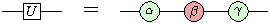
\includegraphics[width=0.5\textwidth]{chapter-2/unitary}
    \caption{Arbitrary single-qubit rotation.}
\end{figure}

The Hadamard gate $H$ corresponds to a rotation of the Bloch sphere $\pi$ radians about the line bisecting the $X$ and $Z$ axes. Up to a global phase of $\text{exp} \left(-i \frac{\pi}{4} \right)$, it can be decomposed using Euler angles by choosing $\alpha = \beta = \gamma = \frac{\pi}{2}$. 

\includezxdiagramtext{figures/chapter-2/hadamard}{0.53}{
\frac{1}{\sqrt 2}
\begin{pmatrix} 1 & 1 \\ 1 & -1 \end{pmatrix}}

There are many equivalent ways of decomposing the Hadamard gate $H$ using Euler angles (see Appendix \ref{appendix-hadamard}). Diagrammatically, applying Hadamard generators to all of the legs of a given spider changes the colour of the spider.

\includezxdiagram{chapter-2/colour_changing}{0.45}

%%%

% \subsection{Conjugate, Transpose and Adjoint}

% We can find the transpose of a ZX diagram by turning all of its inputs into outputs and all of its outputs into inputs whilst preserving the order of their wires.

% \includezxdiagram{chapter-2/transpose}{1}

% We can find the conjugate of a ZX diagram by simply negating the phases of all spiders in the diagram, $\alpha \rightarrow -\alpha, \,\, \beta \rightarrow -\beta, \dots$.

% \includezxdiagram{chapter-2/conjugate}{0.6}

% It is then a simple matter to find the Hermitian adjoint of a ZX diagram by first finding its conjugate, then its transpose.

% \includezxdiagram{chapter-2/adjoint}{0.6}

